\documentclass{article}
\usepackage[utf8]{inputenc}
\usepackage{mathtext}
\usepackage{amsmath}
\usepackage[T1]{fontenc}
\usepackage[utf8]{inputenc}
\usepackage[colorlinks=true, linkcolor=blue]{hyperref}
\usepackage[english, bulgarian, russian]{babel}
\usepackage{tikz}
\usepackage{pgfplots}
\usepackage{indentfirst}
\usepackage[export]{adjustbox}
\usepackage{lipsum} % sample text
\usepackage{floatflt}
\usepackage{multirow}
\usepackage{ textcomp }
\usepackage{geometry} 
\usepackage{animate}
\geometry{verbose,a4paper,tmargin=2cm,bmargin=2cm,lmargin=1.5cm,rmargin=1.5cm}
\setlength{\parindent}{0.65cm}
\setlength{\parskip}{0.15cm}

\usepackage{wrapfig}
\usepackage{array,graphicx,caption}


%Матеша
\usepackage{amsmath,amsfonts,amssymb,amsthm,mathtools} % AMS
\usepackage{icomma} % "Умная" запятая

%\mathtoolsset{showonlyrefs=true} % Показывать номера только у тех формул, на которые есть \eqref{} в тексте.

%% Шрифты
\usepackage{euscript}	 % Шрифт Евклид
\usepackage{mathrsfs} % Красивый матшрифт

%% Свои команды
\DeclareMathOperator{\sgn}{\mathop{sgn}}

%% Перенос знаков в формулах (по Львовскому)
\newcommand*{\hm}[1]{#1\nobreak\discretionary{}
	{\hbox{$\mathsurround=0pt #1$}}{}}
\begin{document}


\begin{titlepage}
     \begin{center}
     \large Московский физико-технический институт\\
    (национальный исследовательский университет)\\
    \vspace{2cm}
    
    \Large Лабораторная работа по курсу  \\  Физические методы исследований\\
    \vspace{2cm}
    { \Huge\bfseries <<ИЗУЧЕНИЕ ЭЛЕКТРОННО-КОЛЕБАТЕЛЬНЫХ СПЕКТРОВ ПОГЛОЩЕНИЯ ДВУХАТОМНЫХ МОЛЕКУЛ НА ПРИМЕРЕ МОЛЕКУЛЫ   $I_2$>> \\ [0.4cm] }
    
     \end{center}
    \vspace{5cm}
    {\par \raggedleft \large Выполнили:\\ студентки 3 курса
    103 группы\\Фитэль Алёна\\ Попеску Полина \par}
    \vspace{3cm}
    \begin{center}
        Долгопрудный, 2024
    \end{center}
\end{titlepage}
\section{Теоретическое введение} 
\subsection{Основы теории молекулярных спектров}
Для большинства практических задач молекулярной спектроскопии достаточно точным является приближённое представление полной волновой функции молекулы в виде произведения
\begin{equation*}
\psi = \psi_{эл(e)} \psi_{кол(\nu)} \psi_{вр(r)},
\end{equation*}
В таком приближении полная энергия молекулы представляется как сумма
\begin{equation*}
E = E_e+ E_{\nu}+E_{r} 
\end{equation*}
Значит измерение полной энергии равно 
\begin{equation*}\Delta E[Дж] = \Delta E_{e} + \Delta E_{\nu} + \Delta E_{r}~ или \end{equation*}
\begin{equation*}v[см^{-1}] =  v_{e} +  v_{\nu} +  v_{r}, \end{equation*}
где разность энергий состояний выражена в волновых числах $v = \frac{\Delta E}{hc} = \lambda^{-1}[см^{-1}]$.

Соотношение между величинами отдельных слагаемых приблизительно равно 
\begin{equation} 
\label{sootnoshenie}
\Delta E_{e}  = \Delta E_{\nu}\cdot 10^3 = \Delta E_{r}\cdot 10^6  \end{equation}

 Электронные переходы в молекуле дают спектры, лежащие в видимой и ультрафиолетовой областях ($\lambda \approx$ 0,1 \textdiv ~1,0 мкм), колебательные спектры расположены в ближней инфракрасной области ($\lambda \approx$ 1 \textdiv ~100 мкм), а чисто вращательные спектры занимают далёкую ИК и субмиллиметровую область ($\lambda \geqslant 100~ мкм$).
 \subsection*{Гармонический осциллятор}
 \begin{figure}[h]
\begin{center}
\begin{minipage}[h]{0.4\linewidth}
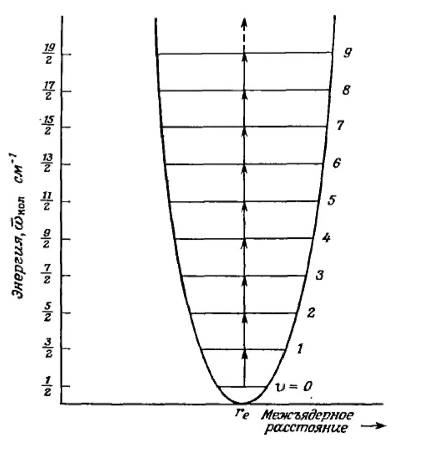
\includegraphics[width=1\linewidth]{Screenshot 2024-02-17 at 3.53.50 PM.png}
\caption{Разрешенные уровни колебательной энергии и некоторые переходы между ними для двухатомной молекулы, испытывающей чисто гармонические колебания}
\label{garm}
\end{minipage}
\hfill 
\begin{minipage}[h]{0.4\linewidth}
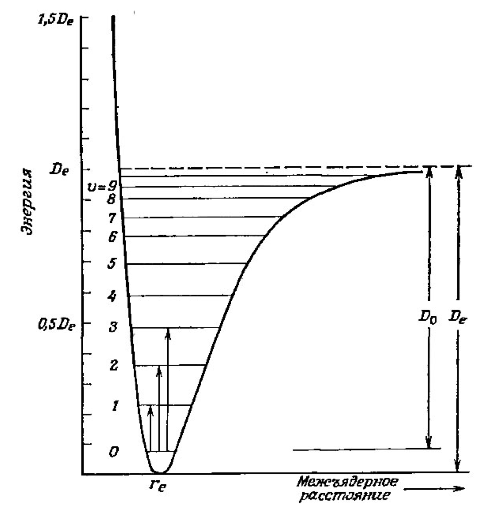
\includegraphics[width=1\linewidth]{Screenshot 2024-02-17 at 3.51.57 PM.png}
\caption{Разрешенные уровни колебательной энергии и некоторые переходы между ними для двухатомной молекулы, совершающей 
ангармонические колебания} %% подпись к рисунку
\label{agarm}
%% метка рисунка для ссылки на него
\end{minipage}


\end{center}
\end{figure}
 Причиной образования из двух атомов ковалентно связанной молекулы можно считать определенную внутреннюю электронную перестройку. С одной стороны, действуют силы отталкивания между одноименными зарядами (положительно заряженные ядра обоих атомов и отрицательные электронные «облака»), с другой – силы притяжения между разноименными зарядами (ядром одного атома и электронами другого и наоборот). 

Поведение связи при сжатии и растяжении можно сравнить с поведением  пружины  и,  продолжая  аналогию,  предположить,  что молекулярная связь подчиняется закону Гука: $f = −k_f (r-r_e )$. В этом случае энергия системы представляет собой параболу и описывается формулой $E = 0.5k_f (r-r_e )^2$.
На \hyperref[garm]{рисунке \ref*{garm}} представлен график энергии, соответствующий этому уравнению.

 Разрешенные значения уровней колебательной энергии в приближении простого гармонического осциллятора можно записать как
 \begin{equation}
     E_{\nu}[Дж] = (\nu +\frac{1}{2})~\omega_e \cdot h c, ~~ \nu = 0,1,2,\dotsb
 \end{equation}
  
 где $\nu$ - колебательное квантовое число, $\omega_e$ - гармоническая частота колебаний $ см^{-1}$, которая является
одной из основных молекулярных констант.


\subsubsection*{Ангармонический осциллятор}
Реальные молекулы не следуют точно законам простого гармонического движения; реальные связи, хотя и упруги, но не столь строго, чтобы  абсолютно  точно  выполнялся  закон  Гука.  Если  достаточно сильно  растягивать  связь  между  атомами,  то  она  в  конце  концов разорвется – молекула диссоциирует на атомы. 

На \hyperref[agarm]{рисунке \ref*{agarm}}  схематично представлена потенциальная энергия в зависимости от межъядерного расстояния для двухатомной молекулы, испытывающей  ангармоническое сжатие  и  растяжение.  

Эмпирическое выражение, которое хорошо описывает кривую этого типа, было получено П.М. Морзе и называется функцией Морзе:

\begin{equation}
\label{morze}
    U(r-r_e) = D_e[1-e^{-\beta(r-r_e)}]^2,
\end{equation}
где $D_e$ - энергия диссоцицации молекулы, отсчитываемая от минимума потенциальной кривой (\hyperref[agarm]{рис. \ref*{agarm}}),  
$\beta = \omega_e\sqrt{(\frac{2\pi ^2 \mu c}{D_e h})}$. \hyperref[morze]{ Потенциальной кривой \ref*{morze}} соответствуют квантованные значения колебательной энергии ангармонического осциллятора 
\begin{equation}
    E_\nu = hc\cdot \{ \omega_e(\nu + \frac{1}{2}) - \omega_e x_e(\nu + \frac{1}{2})^2 \},
\end{equation}
где $x_e$ - коэффициент ангармоничности. 

\subsubsection*{Исследование колебательной структуры}
При исследованиях колебательной структуры можно пренебречь вращательной энергией по сравнению с электронной и колебательной (см. \hyperref[sootnoshenie]{соотношение \ref*{sootnoshenie}}). В этом случае положение полос определяется выражением
\begin{equation}
\label{eq:v(nu)}
    v = v_{эл} + [\omega'_e(\nu'+\frac{1}{2}) - \omega'_e x'_e(\nu'+\frac{1}{2})^2] - [\omega''_e(\nu''+\frac{1}{2}) - \omega''_e x''_e(\nu''+\frac{1}{2})^2]
\end{equation}

Все наблюдаемые в спектре полосы, описываемые уравнением \hyperref[eq:v(nu)]{уравнением \ref*{eq:v(nu)}} можно разбить на две группы серий, или прогрессий. Начиная с некоторого нижнего (верхнего) колебательного уровня $\nu$ , возможны серии переходов на все колебательные уровни верхнего (нижнего) электронного состояния (см. \hyperref[fig:potencialine_krivie]{рис. \ref*{fig:potencialine_krivie}}). Эти серии называются соответственно $\nu'$ и $\nu''$- прогрессиями. Волновые числа наблюдаемых переходов представляются в виде так называемой таблицы Деландра, в столбцах которой располагаются последовательные $\nu'$ -прогрессии, а в строках – $\nu''$ -прогрессии. 
\subsubsection*{Интенсивность  электронно-колебательных  спектров:  принцип Франка–Кондона}
Несмотря на то, что квантовая механика не налагает никаких ограничений на изменение колебательного квантового числа при электронном  переходе,  колебательные  линии  полосы  имеют  неодинаковую интенсивность. 

Экспериментальные  наблюдения  спектров  хорошо объясняются в рамках принципа Франка–Кондона, согласно которому электронный переход происходит настолько быстро, что за время перехода колеблющаяся молекула не успевает заметно изменить свое межъядерное расстояние. 

Отсюда на диаграмме кривых потенциальной энергии квантовые переходы между различными электронными состояниями двухатомной молекулы должны изображаться вертикальными стрелками.

Если верхнее электронное состояние, в которое переходит двухатомная молекула, устойчиво относительно диссоциации на атомы, его можно изобразить другой функцией Морзе, по форме похожей на функцию Морзе основного состояния - см. \hyperref[fig:potencialine_krivie]{рисунок \ref*{fig:potencialine_krivie}}

\begin{figure}[h!]
    \centering
    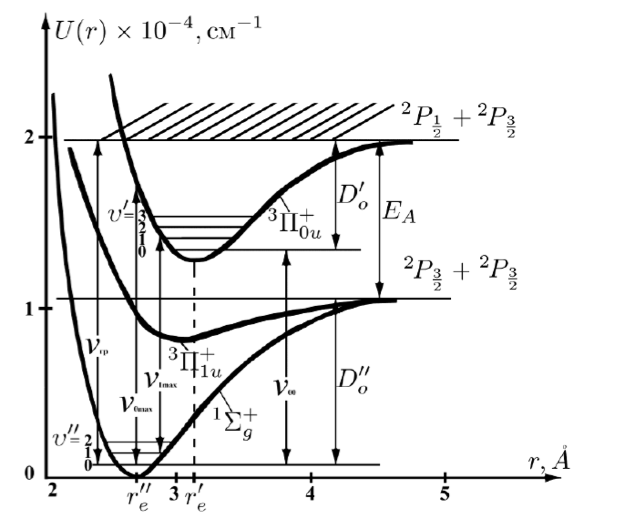
\includegraphics[scale = 0.6]{Screenshot 2024-02-12 at 11.55.07 AM.png}
    \caption{Кривые потенциальной энергии состояний $^1\sum^+_g ,~ ^3П^+_{1u},~ ^3П^+_{0u}$ молекулы $I_2$}
    \label{fig:potencialine_krivie}
\end{figure}
 \newpage
\subsection{Спектр поглощения молекулы $I_2$. Определение молекулярных постоянных.}

В данной работе исследуется электронно-колебательно- вращательный спектр поглощения паров йода. Исследуемый спектр
поглощения соответствует электронному переходу $^1\sum^+_g~ $→ $~^3П^+_{0u}$  и лежит в области длин волн $490 \leqslant \lambda \leqslant 650~ нм$ ($15400 \leqslant v \leqslant 20400 ~см^{−1}$ ).

Если провести анализ колебательной структуры наблюдаемого электронного перехода, т.е. измерить значения волновых чисел полос и произвести их отнесение неопределенным значениям колебателных квантовых чисел $\nu''$  и $\nu'$  нижнего и верхнего электронных состояний, то можно определить коэффициенты \hyperref[eq:v(nu)]{уравнения \ref*{eq:v(nu)}}, и таким образом оценить величины молекулярных постоянных
$T_e, \omega'_e, \omega'_e x'_e, \omega''_e, \omega''_e x''_e$.
\begin{enumerate}
    \item Определение $\omega'_e,~\omega'_e x'_e$. 

    Для этого вычисляют так называемые первые разности $\Delta G'_{\nu'+0.5}$, т.е. разности волновых чисел соседних полос данной прогрессии и анализируют их зависимость от $\nu$. Из
\hyperref[eq:v(nu)]{уравнения \ref*{eq:v(nu)}} при фиксированном $\nu''$ (т.е. для $\nu'$ – прогрессии) имеем
\begin{equation}
\label{eq:G}
    v(\nu'+1)-v(\nu') =  \Delta G'_{\nu'+0.5} = \omega'_e - 2\omega'_e x'_e(\nu'+1)
\end{equation}

\begin{figure}[h]
\begin{center}
\begin{minipage}[h]{0.4\linewidth}
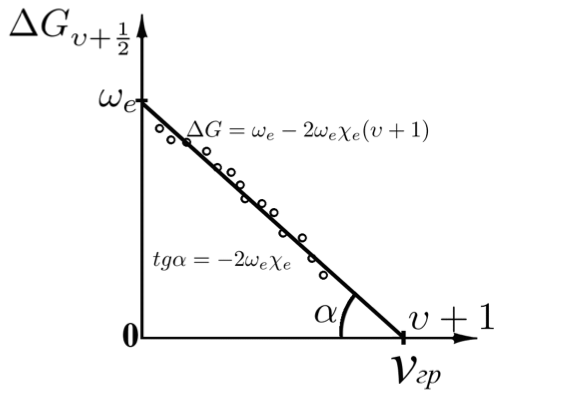
\includegraphics[width=1\linewidth]{Screenshot 2024-02-12 at 11.09.09 AM.png}
\caption{Графическое определение $\omega'_e,~\omega'_e x'_e$ из линейной зависимости $\Delta G'_{\nu'+0.5} ~(\nu'~ +~1)$} %% подпись к рисунку
\label{fig:G(v+1)} %% метка рисунка для ссылки на него
\end{minipage}
\hfill 
\begin{minipage}[h]{0.4\linewidth}
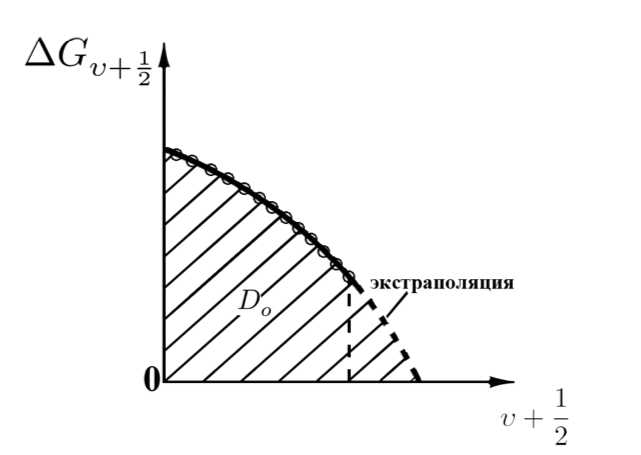
\includegraphics[width=1\linewidth]{Screenshot 2024-02-12 at 1.01.21 PM.png}
\caption{Экстраполяция Берджа - Шнопер}
  \label{fig:berdj-shnoper}
\end{minipage}
\end{center}
\end{figure}

С другой стороны, эти константы можно определить используя зависимость $v_{\nu', \nu''} (\nu')$ (экспериментальные данные) , считая, что она имеет вид $y = A + Bx + CX^2$. Тогда есть согласно \hyperref[eq:v(nu)]{уравнению \ref*{eq:v(nu)}}
\begin{equation}
\label{const}
    x = \nu' + \frac{1}{2},~~A = \nu_{эл} = T_e, ~~B = \omega'_e, ~~ C = -\omega'_e x'_e
\end{equation} 
\item Вычисление $\nu_{гр}$. 

Из \hyperref[eq:G]{уравнения \ref*{eq:G}}, приравняв  $\Delta G'_{\nu'+0.5}$ к нулю (\hyperref[fig:G(v+1)]{рисунок \ref*{fig:G(v+1)}}), можно получить величину $\nu_{гр}$ , т.е. колебательное квантовое число «последнего» дискретного уровня колебательной энергии, граничащего со
сплошным спектром. Молекула, которой сообщена энергия выше
уровня, определяемого величиной $\nu_{гр}$ , диссоциирует. 

Однако, как правило,
даже при наличии на спектрограмме участка перехода системы полос в сплошной спектр для нахождения величины $v_{гр}$ требуется дополнительная экстраполяция. 

Если пренебречь ангармоничностью более высокого порядка чем $\omega_e x_e$, то из \hyperref[eq:v(nu)]{уравнения \ref*{eq:v(nu)}} можно получить, что зависимость $v$ от $\Delta v = v(\nu'+1)- v(\nu')$ имеет вид
\begin{equation}
\label{v(v)}
    v = a + b\Delta v + c(\Delta v)^2
\end{equation}

При $\Delta v = 0$ коэффициент a в  \hyperref[v(v)]{уравнении \ref*{v(v)}}  вида и есть $v_{гр}$.

\item Определение энергии диссоциации возбужденного и основного уровней

Видно, что сумма разностей соседних колебательных термов, начиная с $\nu = 0$ до $\nu_{гр}$ , равна энергии диссоциации для данного электронного состояния

\begin{equation}
\label{D0 berdj shnop}
    \sum_{\nu = 0}^{\nu = \nu_{гр}} \Delta G'_{\nu'+0.5} = D_0
\end{equation}

В \hyperref[eq:G]{приближении \ref*{eq:G}} энергия диссоциации равна 
\begin{equation}
\label{eq:D0 lin}
    D'_0 = \frac{\omega^2_e}{4\omega_e x_e}
\end{equation}

С другой стороны, более точно можно определить энергию
диссоциации методом графической экстраполяции Берджа-Шпонер. Строится график зависимости наблюдаемых колебательных
интервалов $\Delta G'_{\nu'+0.5}$ от $\nu + \frac{1}{1}$ , который экстраполируется до пересечения с осью абсцисс (\hyperref[fig:berdj-shnoper]{рисунок \ref*{fig:berdj-shnoper}}). Согласно уравнению \hyperref[D0 berdj shnop]{рисунок \ref*{D0 berdj shnop}} площадь под этой кривой соответствует энергии диссоциации. 

Также из \hyperref[fig:potencialine_krivie]{рисунок \ref*{fig:potencialine_krivie}} $D'_0 = v_{гр} - v_{00}$, а $D''_0 = v_{гр} - E_A $ (где для атома йода $E_A = 7603 ~см^{-1}$) 



\item Определение $r'_e$ - межъядерного расстояния в возбужденном состоянии.

Обозначим $v_{max}$ - волновое число полосы с максимальным поглощением $\nu'' = 0$ → $\nu'_{max}$. Тогда потенциальная энергия, отсчитывуаемая от минимума верхней потенциальной кривой равна 
\begin{equation}
\label{U1}
    U'(r' = r''_e) = v_{max} - v_{00} + \frac{\omega'_e}{2}
\end{equation}

С другой стороны, по \hyperref[morze]{ формуле Морзе \ref*{morze}} для верхнего состояния 
\begin{equation}
\label{U2}
    U'(r' = r''_e) = D'_e\left[1- \exp(-\beta'(r''_e-r'_e))\right] ^2,
\end{equation}
где $D'_e = D'_0 + \frac{\omega'_e}{2}, ~\beta' = w'_e\sqrt{(\frac{2\pi ^2 \mu c}{D'_e h})}\approx 0,12177 w'_e \sqrt{\frac{\mu}{D'_e}}$

\begin{equation}
\label{r'e}
    \Rightarrow r'_e-r''_e = \frac{1}{\beta'}\ln\left[1+\left(\frac{U'(r' = r''_e)}{D'_e}\right)^{1/2}\right]
\end{equation}

Отсюда, зная $r''_e$ определяют $r'_e$ 
\end{enumerate}


\section{Выполнение задания} 


\subsection{Проведение эксперимента}

В данной работе регистрация спектров поглощения паров йода производится с помощью автоматического спектрофотометра для видимой и ультрафиолетовой областей «Specord M400». Оптическая схема прибора приведена на \hyperref[fig:ustanovka]{рисунке \ref*{fig:ustanovka}} в конце отчета.


Для наблюдения изменения характера спектра при изменении температуры цилиндрическая стеклянная кювета с кристаллами йода устанавливается в кюветном отсеке прибора с помощью специального держателя, который нагревается до необходимой температуры водой, подаваемой по соединительным шлангам от термостата - см. схему на \hyperref[fig:ustanovka2]{рисунке \ref*{fig:ustanovka2}}.


\begin{figure}[h!]
    \centering
    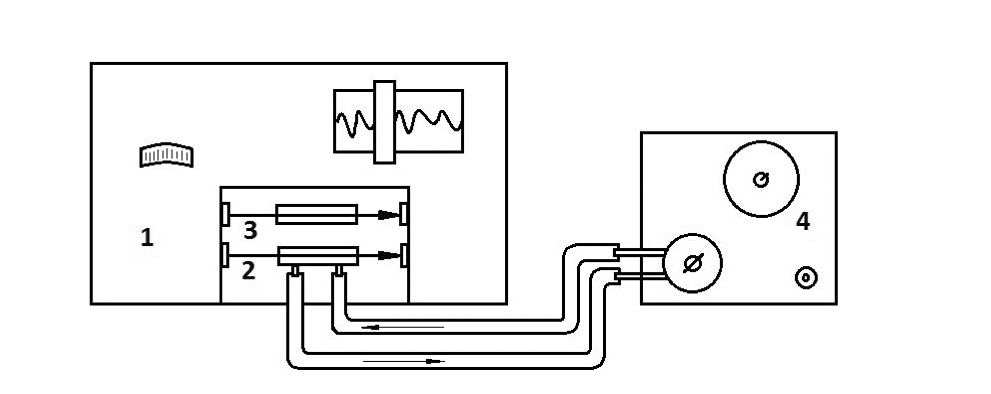
\includegraphics[scale=0.3]{Screenshot 2024-02-12 at 10.12.27 AM.png}
    \caption{Схема установки: 1 – корпус спектрометра, 2 – кювета с парами йода, 3 – кювета сравнения, 4 – термостат}
    \label{fig:ustanovka2}
\end{figure}





\begin{enumerate}
    \item Для спектрального диапазона $\lambda = 480 \div 655~нм$, шага сканирования 0.2 нм, ширине щели 0.1 нм, скорости сканирования $\frac{d\lambda}{dt} = 0.5~нм/с$ снимем спектры при трех температурах: 40°С, 55°С и 70°С. 
    
    Изобразим на \hyperref[fig:I2(40)]{рисунке \ref*{fig:I2(40,50,70)}} полученные спектры при данных температурах. При более высокой температуре амплитуда спектра больше, то есть интенсивность поглощения увеличивается.
\begin{figure}[h!]
    \centering
    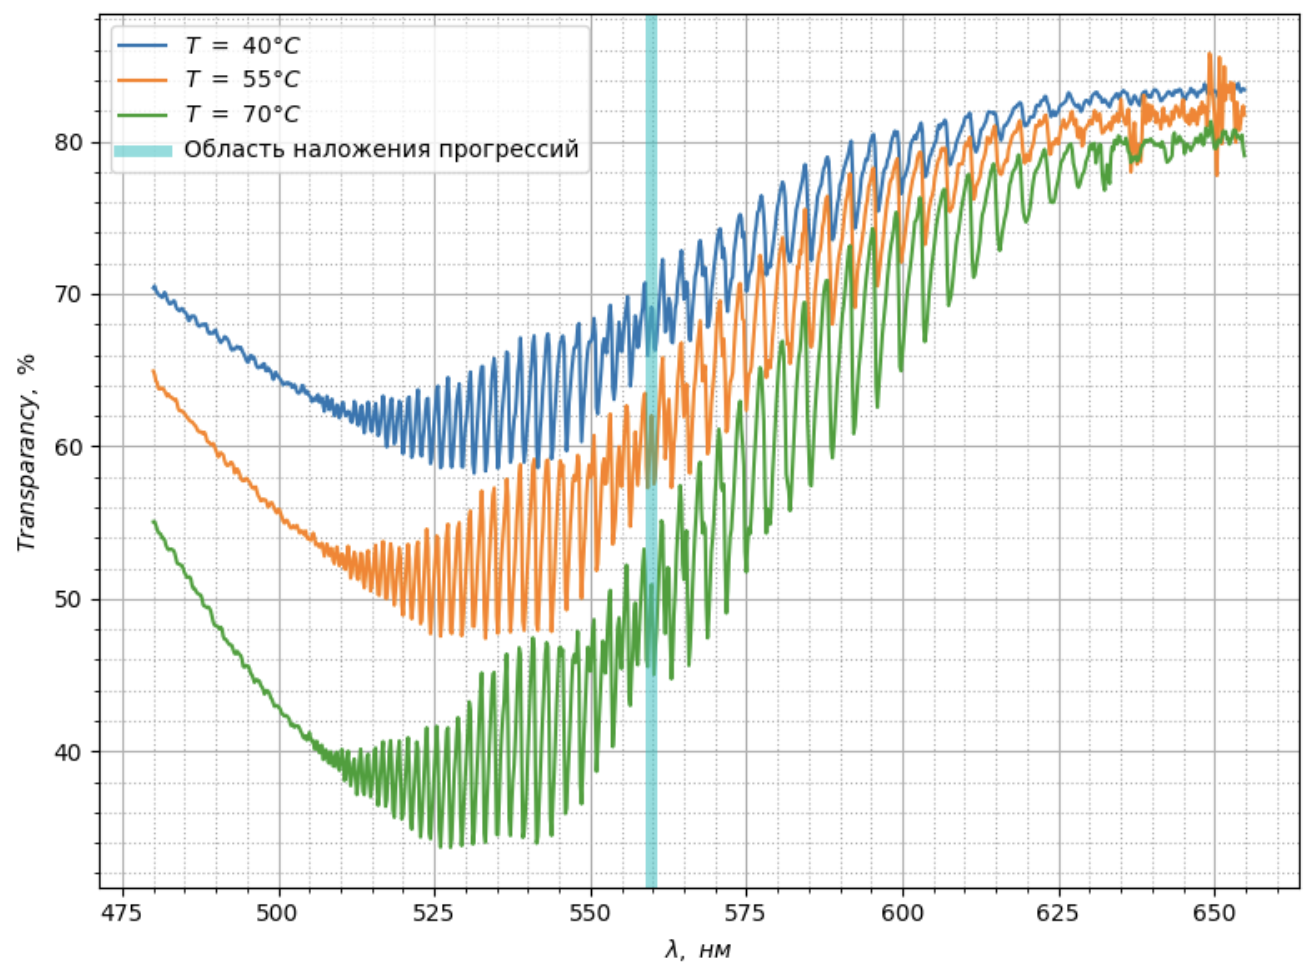
\includegraphics[scale = 0.55]{i2_405570.png}
    \caption{Спектр прозрачности паров йода при различных температурах}
    \label{fig:I2(40,50,70)}
\end{figure}
\newpage
\item Для температуры 70°С произведем измерения спектра при трех ширинах щели: 0.1 нм, 1 нм и 5 нм. Полученные зависимости приведены на \hyperref[fig:I2(70)]{рисунке \ref*{fig:I2(70)}}: 
\begin{figure}[h!]
    \centering
    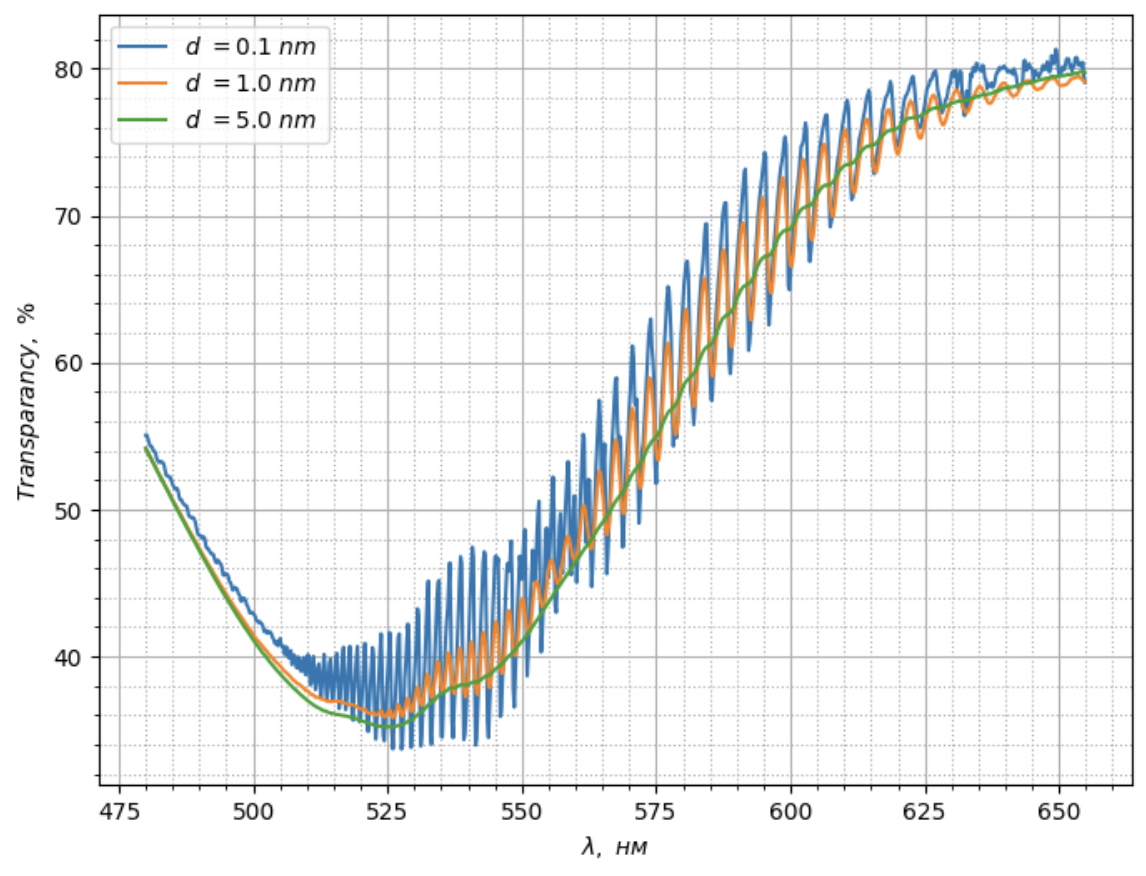
\includegraphics[scale = 0.55]{щель_new.png}
    \caption{Спектр прозрачности паров йода при различной величине щели при температуре 70°С}
    \label{fig:I2(70)}
\end{figure}

При увеличении ширины щели амплитуда пиков уменьшается, при $d = 5.0 нм$ часть пиков не видна совсем. Это связано с тем, что при увеличении ширины щели увеличивается степень немонохроматичности света, падающего на кювету с парами йода, и пики "усредняются" на большем интервале $[\lambda - \Delta \lambda, \lambda + \Delta \lambda]$.
\item При температуре 70°С для ширины в 0.1 нм снимем спектр в диапазоне длин волн $\lambda = 340 \div 700~нм$ - см. \hyperref[fig:I2(70-wide)]{рисунок \ref*{fig:I2(70-wide)}}.
\begin{figure}[h!]
    \centering
    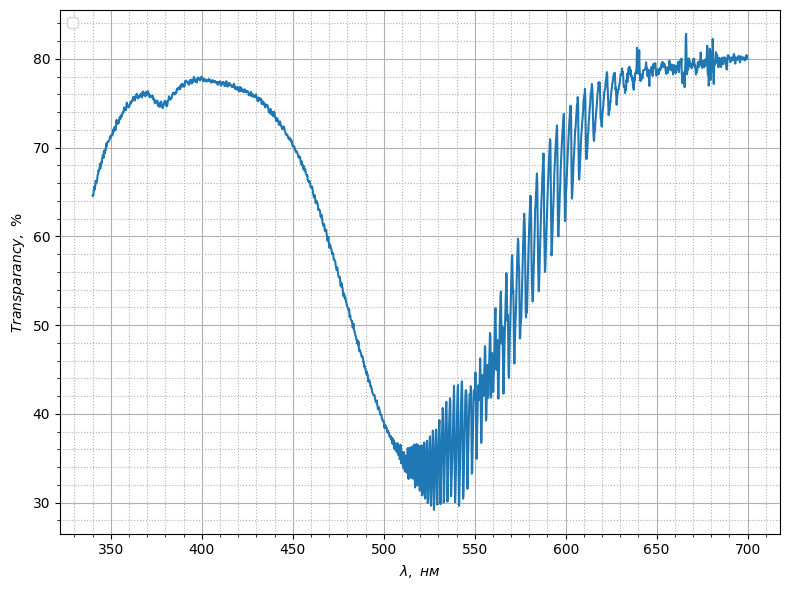
\includegraphics[scale = 0.6]{I2(70-wide).png}
    \caption{Спектр прозрачности паров йода при температуре 70°С в более широком диапазоне длин волн}
    \label{fig:I2(70-wide)}
\end{figure}
\newpage
\item Далее будем обсчитывать спектр при 40°С, так как при этой температуре уже достигается достаточная плотность паров йода, но еще мала населенность колебательных уровней $\nu ''~\geqslant ~2$ основного электронного состояния. Поэтому можно считать, что в спектре присутствуют только 2 прогрессии:
$\nu ''$ = 1 → $\nu '$ (правая – низкочастотная) и $\nu ''$ = 0 → $\nu '$ (левая – высокочастотная). Выделим полосы, относящиеся к этим прогрессиям и проведем отнесение полос спектра - \hyperref[fig:I2(40)]{рисунок \ref*{fig:I2(40)}}, составим \hyperref[tab:delandra]{таблицу Деландра \ref*{tab:delandra}} - см. конец работы.
\begin{figure}[h!]
    \centering
    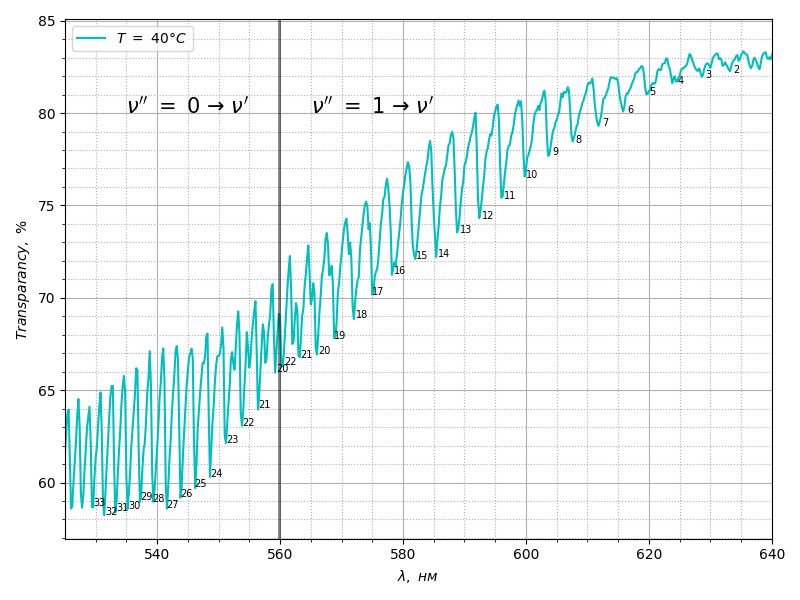
\includegraphics[scale = 0.7]{I2(40).png}
    \caption{Отнесение полос спектра при T = 40°С}
    \label{fig:I2(40)}
\end{figure}


\item Вычислим разности соседних волновых чисел в полученных $\nu'$- прогрессиях $v(\nu' +1)- v(\nu) = \Delta G'_{\nu'+0.5}$. Занесем их в \hyperref[tab:delandra]{таблицу \ref*{tab:delandra}}.
\item Используя полученные значения $\Delta G'_{\nu'+0.5}$ определим $\omega'_e,~\omega'_e x'_e$ из угла наклона \hyperref[fig:G(nu)]{графика \ref*{fig:G(nu)}}  $\Delta G'_{\nu' +0.5}~ (\nu'~ +~1)$ (см. \hyperref[fig:G(v+1)]{рисунок \ref*{fig:G(v+1)}})

 \begin{figure}[h!]
     \centering
     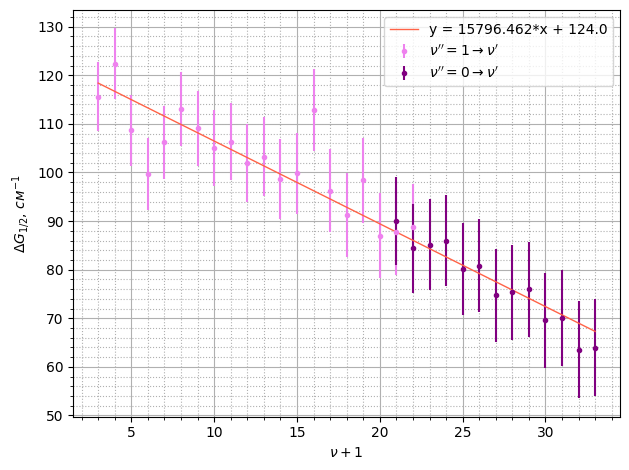
\includegraphics[scale = 0.9]{I2-linear2.png}
     \caption{Зависимость первых разностей от колебательного квантового числа возбужденного состояния}
     \label{fig:G(nu)}
 \end{figure}

 \begin{equation*}
     \fbox { b = \omega'_e = 123.1 \pm 2.1~см^{-1}, ~~-\frac{k}{2} =  \omega'_e x'_e = 0.84 \pm 0.05~см^{-1}}
 \end{equation*}
\item  Используя \hyperref[const]{соотношения \ref*{const}}, определим значение $\omega'_e,~\omega'_e x'_e$ и $T_e$ возбужденного состояния $^3П^+_{0u}$ из \hyperref[fig:v(nu)]{графика \ref*{fig:v(nu)}} $y (\nu' + 1/2)$, где 

\begin{equation*}
y = 
\left\{ \begin{aligned} 
  v_{0, \nu'} + \frac{1}{2}\omega_e'',\text{ }\nu'' = 0\\
  v_{0, \nu'} + \frac{3}{2}\omega_e'', \text{ }\nu'' = 1,
\end{aligned} \right.
\end{equation*}
$\omega_e'' = 214.5 см^{-1}$:
\begin{figure}[h!]
    \centering
    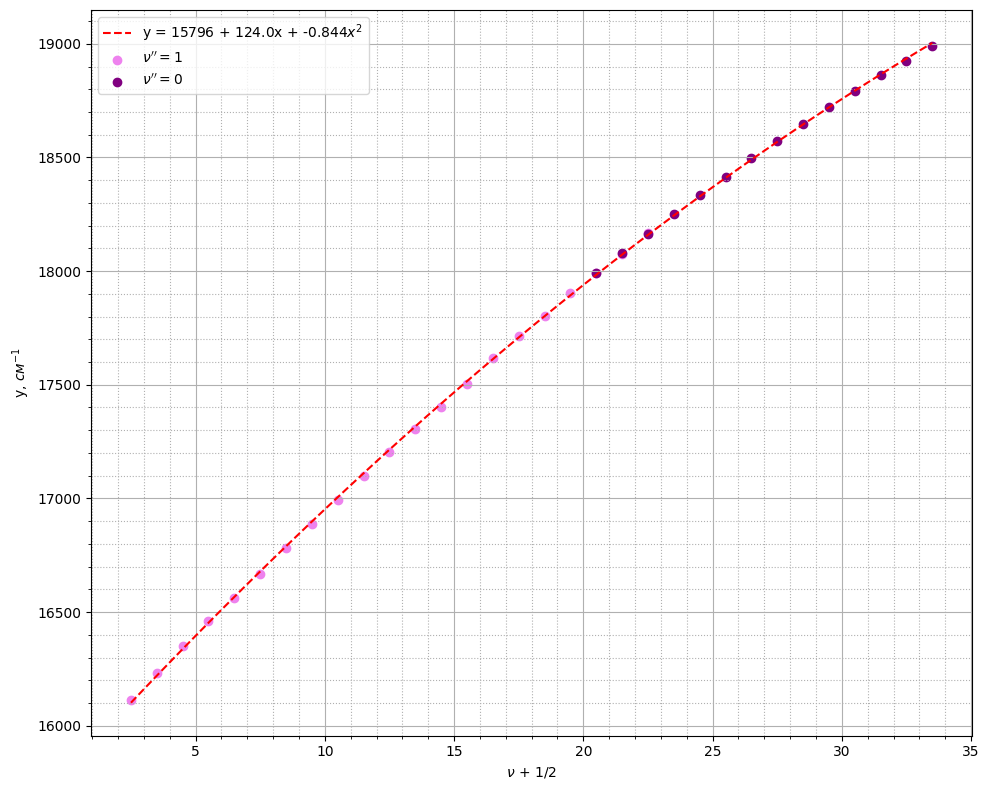
\includegraphics[scale = 0.6]{I2-parabola.png}
    \caption{Зависимость волнового числа от колебательного квантового числа возбужденного
состояния}
    \label{fig:v(nu)}
\end{figure}
\begin{equation*}
    \fbox {A = v_{эл} = T_e = 15796 \pm 6 ~см^{-1}, ~~B = \omega'_e = 124.0 \pm 0.7 ~см^{-1},  ~~ C = -\omega'_e x'_e = -0.84 \pm 0.02 ~см^{-1}}
\end{equation*} 
\item Вычислим волновое число $v_{0,0} = T_e + 0.5\omega'_e - 0.5w''_e$ (см. \hyperref[fig:potencialine_krivie]{рисунок \ref*{fig:potencialine_krivie}})
\begin{equation*}
\underline {v_{0,0} = (15751 \pm 6) ~см^{-1}}
\end{equation*}

\item Определим $v_{гр}$. Для этого, считая, что волновые числа полос $v(\nu')$ и их разности $\Delta v = v(\nu'+1)-v(\nu')$ связаны \hyperref[v(v)]{квадратичой зависимостью \ref*{v(v)}} для переходов $\nu'' = 0 $→ $\nu'$, построим график зависимости:

\begin{figure}[h!]
    \centering
    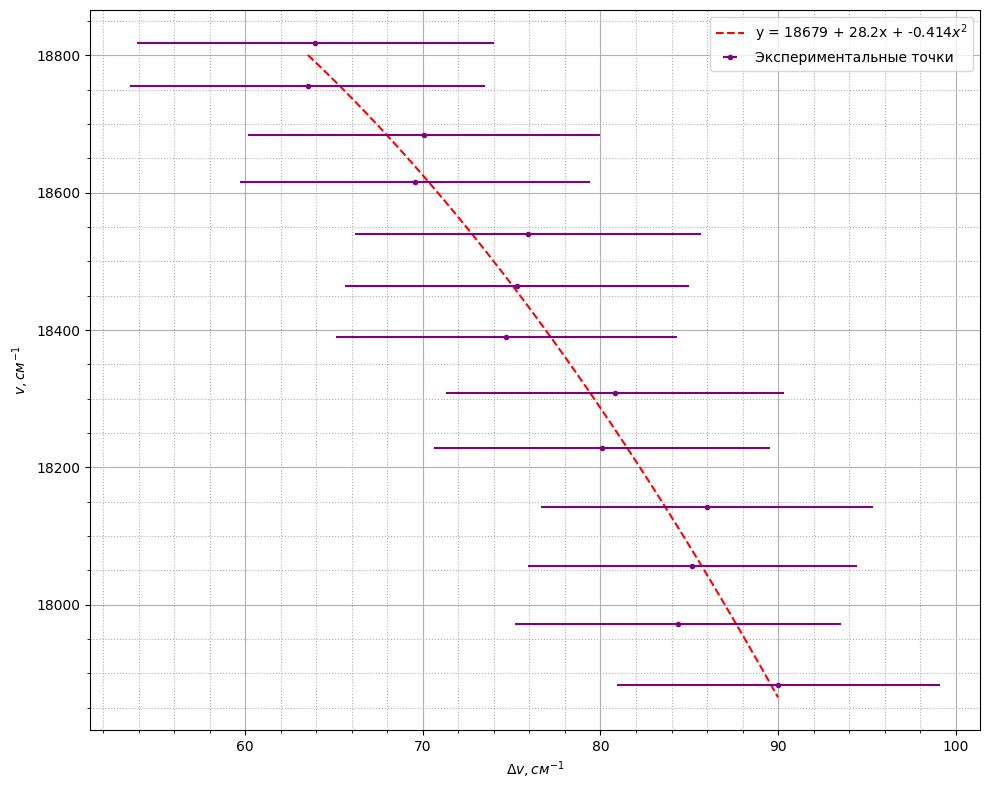
\includegraphics[scale = 0.5]{I2-granitsa.png}
    \caption{Зависимость волновых чисел от первых разностей при $\nu''=0$}
    \label{fig:I2-gr}
\end{figure}
Из коэффициентов регрессии найдем значение $v_{гр}$:
\begin{equation*}
    \underline{ A = v_{гр} = 19000 \pm 2000 ~см^{-1}}
\end{equation*}

\item Используя полученные в предыдущих пунктах значения молекулярных постоянных, определим энергию диссоциации $D'_0$ для состояния $^3П^+_{0u}$:
\begin{enumerate}
    \item по \hyperref[eq:D0 lin]{формуле линейной экстраполяции \ref*{eq:D0 lin}}
    \begin{equation}
    \label{res:Do}
         \fbox{D'_0 = \frac{\omega'^2_e}{4\omega'_e x'_e} = \frac{124.0^2}{4\cdot 0.84} = 4576,2 \pm 52,7~см^{-1}}
    \end{equation}
    \begin{equation*}
        \delta D'_0 = \sqrt{\left(2\frac{\omega'_e}{4\omega'_e x'_e}\cdot \delta \omega'_e\right)^2 + \left (\frac{\omega'^2_e}{4(\omega'_e x'_e)^2}\cdot \delta (\omega'_e x'_e)\right) ^2} = 52,7~см^{-1}
    \end{equation*}
    \item по границе сплошного спектра (\hyperref[fig:potencialine_krivie]{рис. \ref*{fig:potencialine_krivie}})
    \begin{equation}
        \label{res1:Do}
        \fbox{D'_0 = v_{гр} - v_{00} = 19000-15751 = 3249 \pm 2000~см^{-1}}
    \end{equation}
    \item Методом экстраполяции Берджа-Шнопера. Для этого строим график зависимости колебательных интервалов \hyperref[fig:I2-berdg]{$\Delta G'_{\nu'+0.5} ~(\nu' +0.5)$ \ref*{fig:I2-berdg}}, который экстраполируется до пересечения с осью абсцисс - \hyperref[fig:berdj-shnoper]{рис. \ref*{fig:berdj-shnoper}}. 
    \begin{figure}[h!]
    \centering
    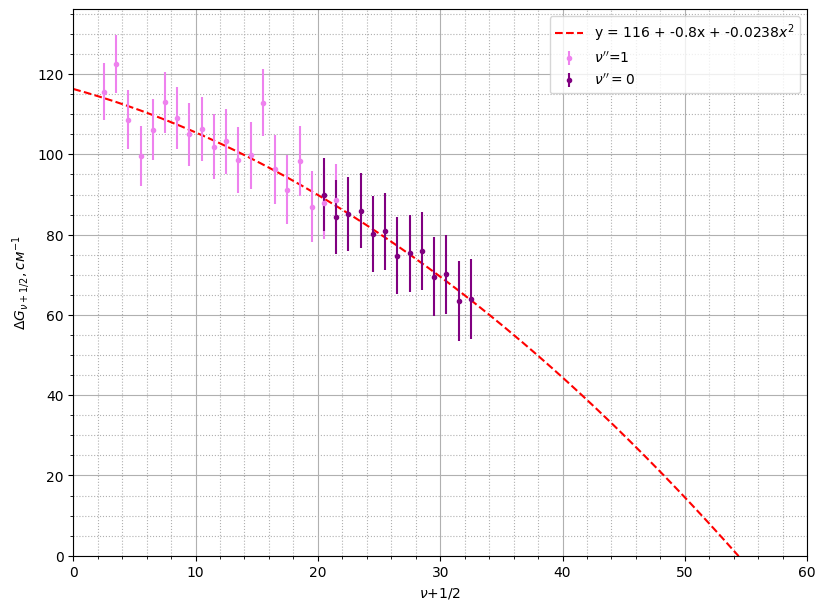
\includegraphics[scale = 0.5]{I2-Berdg.png}
    \caption{Экстраполяция Берджа-Шпонер}
    \label{fig:I2-berdg}
\end{figure}
Коэффициенты апроксимации параболой:
\begin{equation*}
    a = 116 \pm 5~см^{-1},\text{  } b= -0.8 \pm 0.5~см^{-1},\text{  } c = -0.024 \pm 0.012~см^{-1} 
\end{equation*}
    Согласно \hyperref[D0 berdj shnop]{уравнению \ref*{D0 berdj shnop}} площадь под этой кривой соответствует энергии диссоциации, то есть
    \begin{equation*}
         для~y = \Delta G'_{\nu'+0.5}, ~~ x = \nu'+0.5,~~имеем~ y = cx^2+bx+a,~пересекающую ~ось~ абсцисс~ в ~x_0 = 54,8
    \end{equation*}
    \begin{equation*}
    \Rightarrow \fbox{ D'_0= \frac{c x_0^3}{3}+\frac{b x_0^2}{2}+a x_0 = 3939,1\pm 1035,4~см^{-1}}
    \end{equation*}
    \begin{equation*}
        \delta D'_0 = \sqrt{\left( \frac{x_0^3}{3}\cdot \delta c\right)^2+\left( \frac{x_0^2}{2}\cdot \delta b\right)^2 + \left(x_0 \cdot \delta a\right)^2} = 1035,4~см^{-1} 
    \end{equation*}
\end{enumerate}
 Определим энергию диссоциции основного состояния $^1\sum^+_g$ 
 \begin{equation*}
     \fbox{D''_0 = v_{гр} - E_a = 19000 - 7603 = 11397 \pm 2000~см^{-1}} 
 \end{equation*}
 \item Для прогресии с $\nu'' = 0$ определим волновое число полосы с максимальным поглощением $\underline{v_{max} = 18818.22~см^{-1}}$ (минимум на графике пропускания достигается при $\nu' = 32$). 
 \item Определим равновесное межъядерное расстояние $r'_e$ для возбужденного состояния $^3П^+_{0u}$ используя полученные значения $v_{max}, \omega'_e = 124,0 \pm 0,7~см^{-1}, D'_0 = 4576,2 \pm 52,7~см^{-1}, r''_e = 2,67 \text{\AA}$ и уравнения \hyperref[U1]{ \ref*{U1}}, \hyperref[r'e]{ \ref*{r'e}}
 \begin{equation*}
     \underline{U'(r'= r''_e)} = v_{max} - v_{00} + \frac{\omega'_e}{2} = 18818.22 - 15751 + \frac{124.0}{2} = \underline{3129 \pm 6~см^{-1}}
 \end{equation*}
 \begin{equation*}
     \underline{D'_e} = D'_0 + \frac{\omega'_e}{2} =  4576,2 + \frac{ 124,0}{2} = \underline{4638,2 \pm 52,7~см^{-1}}
 \end{equation*}
 \begin{equation*}
     \underline{\beta'} \approx 0,12177 w'_e \sqrt{\frac{\mu}{D'_e}} =  0,12177\cdot 124,0 \sqrt{\frac{63.5~а. ~е. ~м.}{4638,2}} = \underline{1,77\pm 0,01~\text{\AA}^{-1}}
 \end{equation*}
 \begin{equation*}
     \delta \beta' = 0,12177\sqrt{\left(\frac{\mu}{D'_e}\cdot (\delta w'_e)^2 \right)+ \left( w'_e \cdot \frac{1}{2}\sqrt{\frac{\mu}{D'_e^3} }\cdot \delta D'_e \right)^2} = 0,01~\text{\AA}^{-1}
 \end{equation*}
 \begin{equation*}
     \underline{r'_e} = r''_e + \frac{1}{\beta'}\ln\left[1+\left(\frac{U'(r' = r''_e)}{D'_e}\right)^{1/2}\right] = 2,67 +  \frac{1}{1,77}\ln\left[1+\left(\frac{3129}{4638,2}\right)^{1/2}\right] = \underline{3,01\pm0,06~\text{\AA} }
 \end{equation*}
 \begin{equation*}
     \delta r'_e = \sqrt{\left(\frac{\ln\left[1+\left(\frac{U'(r' = r''_e)}{D'_e}\right)^{1/2}\right]}{\beta'^2}\cdot \delta \beta'\right) ^2+\left(\frac{1}{\beta'}\frac{1}{\left[1+\left(\frac{U'(r' = r''_e)}{D'_e}\right)^{1/2}\right]}\frac{1}{2} \left(\frac{1}{U'(r' = r''_e)\cdot D'_e}\right)^{1/2} \cdot \delta U'(r' = r''_e)\right)^2 +}
 \end{equation*}
 \begin{equation*}
 \overline{+ \left(\frac{1}{\beta'}\frac{1}{\left[1+\left(\frac{U'(r' = r''_e)}{D'_e}\right)^{1/2}\right]}\frac{1}{2} \left(\frac{U'(r' = r''_e)}{D'_e^3}\right)^{1/2} \cdot \delta D'_e\right)^2} = 0,06~\text{\AA}
 \end{equation*}
 \newpage
 \item Построим \hyperref[fig:morze]{потенциальную кривую  \ref*{fig:morze}} возбужденного электронного состояния $^3П^+_{0u}$, используя \hyperref[morze]{функцию Морзе \ref*{morze}} 
 \begin{figure}[h!]
     \centering
     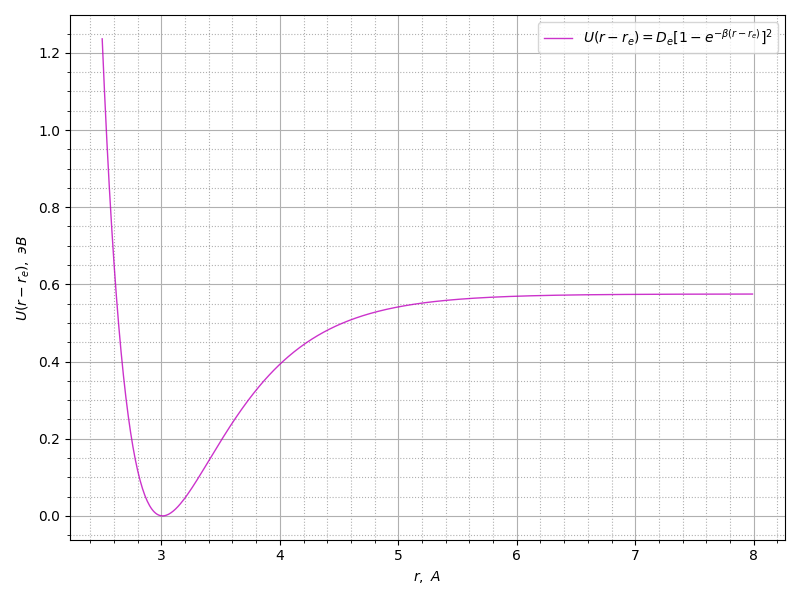
\includegraphics[scale = 0.8]{morze.png}
     \caption{Потенциальная кривая возбужденного электронного состояния $^3П^+_{0u}$}
     \label{fig:morze}
 \end{figure}
\end{enumerate}

 \newpage
\section{Результаты}

В данной работе мы экспериментально получили спектр поглощения паров $I_2$ в \hyperref[fig:I2(40)]{видимой (\ref*{fig:I2(40,50,70)})} и \hyperref[fig:I2(70-wide)]{ультрафиолетовой (\ref*{fig:I2(70-wide)})} областях. Затем для дальнейших рассчетов \hyperref[fig:I2(40)]{сопоставили}  максимумы поглощения с прогрессиями $\nu ''$ = 1 → $\nu '$ и $\nu ''$ = 0 → $\nu '$ при T = 40°С, заполнили \hyperref[tab:delandra]{таблицу Деландра \ref*{tab:delandra}}. 

Построив линейную аппроксимацию \hyperref[fig:G(nu)]{ $\Delta G'_{\nu' +0.5}~ (\nu'+1)$ }  зависимости первых разностей волновых чисел от колебательного квантового числа, первым способом определили $\omega'_e,~\omega'_e x'_e$. Второй способ - с помощью квадратичной аппроксимации \hyperref[fig:v(nu)]{ $v_{\nu', \nu''} (\nu'+1/2)$ }. Полученные данные представлены в \hyperref[tab:results1]{итоговой таблице \ref*{tab:results1}}.  Здесь мы также определили $T_e = 15796 \pm 6~ см^{-1}$.

Далее, для рассчета энергии диссоциации $D'_0$ для состояния $^3П^+_{0u}$ по границе сплошного спектра, мы посчитали волновые числа $v_{0,0} = 15751 \pm 6 ~см^{-1}$, $v_{гр} = 19000 \pm 2000 ~см^{-1}$.

Используя полученные в предыдущих пунктах значения молекулярных постоянных определили $D'_0$ тремя способами - по формуле линейной экстраполяции - \hyperref[res:Do]{ выражение \ref*{res:Do}}, по границе сплошного спектра - \hyperref[res1:Do]{ выражение \ref*{res1:Do}} и по графику \hyperref[fig:I2-berdg]{$\Delta G'_{\nu'+0.5} ~(\nu' +0.5)$ } - методом Берджа-Шнопер. См. \hyperref[tab:results2]{итоговую таблицу \ref*{tab:results2}}. По границе сплошного спектра мы также определили $D''_0 = 11397 \pm 2000~см^{-1}$.

Затем мы оценили межъядерное расстояние $r'_e = 3,01\pm0,06~\text{\AA}$ для возбужденного состояния $^3П^+_{0u}$. Для этого посчитали $v_{max} = 18818.22~см^{-1}$, $U'(r'= r''_e) = 3129 \pm 6~см^{-1}$, $D'_e = 4638,2 \pm 52,7~см^{-1}$, $\beta' = 1,77\pm 0,01~\text{\AA}^{-1}$. 


\begin{table}[h!]
    \centering
    \begin{tabular}{|l|c|c|c|c|} \hline  
               \multicolumn{5}{|r|}{Экспериментальные данные}\\ \hline  
           Молекулярные постоянные&$T_e,~см^{-1}$&  $\omega'_e,~см^{-1}$&  $\omega'_e x'_e,~см^{-1}$&  $r'_e$,~\(\text{\AA}\)\\ \hline  
               Лин. аппроксимация $\Delta G'_{\nu'+0.5}$&-&  $123.1 \pm 2.1$&  $0.84 \pm 0.05$&  -\\ \hline  
               Квадр. аппроскимация  $y (\nu' + 1/2)$&$15796 \pm 6$&  $124.0 \pm 0.7$&  $0.844 \pm 0.020$&  -\\ \hline 
 Через функцию Морзе& -& -& -&$3,01 \pm 0,06 $\\\hline \hline  
               \multicolumn{5}{|r|}{Табличные данные}\\ \hline  
               &15770,6&  125,3&  0,702&  3,028\\ \hline 
    \end{tabular}
   
    \caption  {Результаты определения молекулярных постоянных разными методами}
    \label{tab:results1}
\end{table}

\begin{table}[h!]
    \centering
    \begin{tabular}{|l|c|c|} \hline 
         \multicolumn{3}{|r|}{Экспериментальные данные}\\ \hline 
         Энергия диссоциации&  $D'_0,~см^{-1}; ~эВ$& $D''_0,~см^{-1};~эВ$\\ \hline 
         Лин. экстраполяция&  $4576,2 \pm 52,7$; 0.567 $\pm$ 0.007& -\\ \hline 
         По границе сплошного спектра $D'_0 = v_{гр} - v_{00}$&  $3249 \pm 2000$; 0,403 $\pm$ 0,248& $11397 \pm 2000$; 1,413 $\pm$  0,248\\ \hline 
 Экстрапол. Берджа-Шнопер $\Delta G'_{\nu'+0.5} ~(\nu' +0.5)$& $3939,1\pm1035,4$; 0,488 $\pm$ 0,128&-\\\hline \hline 
         \multicolumn{3}{|r|}{Табличные данные}\\ \hline 
         &  4320; 0,536& 12440;  1,542\\ \hline
    \end{tabular}
    \caption{Результаты определения энергии диссоциации молекулы $I_2$ разными методами}
    \label{tab:results2}
\end{table}

\section{Вывод} 

Проанализируем результаты. 

$T_e$, $\omega'_e,~\omega'_e x'_e$,$r'_e$ вышли близкими к теоретическим. Метод с квадратичной аппроксимацией $v_{\nu', \nu''} (\nu'+1/2)$ дал на порядок меньшую погрешность, чем c линейной $\Delta G'_{\nu'+0.5} ~(\nu' +0.5)$.  

Наиболее близкое к теории и и с наименьшей погрешностью значение дала \hyperref[eq:D0 lin]{формула линейной экстраполяции \ref*{eq:D0 lin}} определения энергии диссоциации. В методе Берджа-Шопер значение вышло меньше теоретического, а ошибка составила 25 $\%$. Хуже всего себя показал метод определения по границе сплошного спектра. Ошибка составляет 60$\%$ самой величины. 

Расхождения в значениях полученных величин определяются неточностью в определении положения пиков поглощения. Также скорее всего, можно было уменьшить погрешность в вычислении некоторых величин, проведя рассчеты для большего числа пиков поглощения.
\newpage
\begin{figure}[h!]
    \centering
    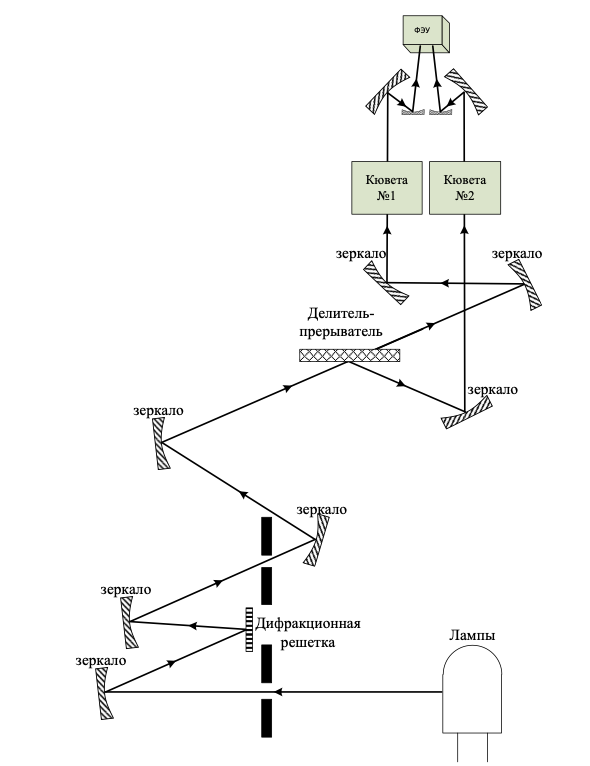
\includegraphics[scale=0.55]{Screenshot 2024-02-12 at 10.10.01 AM.png}
    \caption{Оптическая схема прибора}
    \label{fig:ustanovka}
\end{figure}
\newpage
\begin{table}[h!]
    \centering
    \caption{Таблица Деландра}
    \begin{tabular}{|c|c|c|c|c|} \hline 
          $\nu '/  \nu ''$&  \multicolumn{2}{|c|}{0}&\multicolumn{2}{|c|}{1}\\ \hline 
         &  $\lambda,~nm$&  $\nu, ~cm^{-1}$ &$\lambda,~nm$&  $\nu, ~cm^{-1}$\\ \hline 
         2&  -
&   -
&633,2&  15792,80\\ \hline 
         3&  -
&   -
&628,6&  15908,37\\ \hline 
         4&  -
&   -
&623,8&  16030,78\\ \hline 
         5&  -
&   -
&619,6&  16139,44\\ \hline 
         6&  -
&   -
&615,8&  16239,04\\ \hline 
         7&  -
&   -
&611,8&  16345,21\\ \hline 
         8&  -
&   -
&607,6&  16458,20\\ \hline 
         9&  -
&   -
&603,6&  16567,26\\ \hline
 10& -
& -
& 599,8& 16672,22\\\hline
 11& -
& -
& 596,0& 16778,52\\\hline
 12& -
& -
& 592,4& 16880,49\\\hline
 13& -
& -
& 588,8& 16983,70\\\hline
 14& -
& -
& 585,4& 17082,34\\\hline
 15
& -
& -
& 582,0& 17182,13\\\hline
 16
& -
& -
& 578,2& 17295,05\\\hline
 17
& -
& -
& 575,0& 17391,30\\\hline
 18
& -
& -
& 572,0& 17482,52\\\hline
 19
& -& -& 568,8
& 17580,87\\\hline
 20
& 559,2& 17882,69& 566,0& 17667,84\\\hline
 21
& 556,4& 17972,68& 563,2& 17755,68\\\hline
 22& 553,8& 18057,06& 560,4& 17844,40\\\hline
 23& 551,2& 18142,23& -
& -
\\\hline
 24& 548,6& 18228,22& -
& -
\\\hline
 25& 546,2& 18308,31& -
& -
\\\hline
 26& 543,8
& 18389,11& -
& -
\\\hline
 27& 541,6
& 18463,81& -
& -
\\\hline
 28& 539,4& 18539,12& -
& -
\\\hline
 29& 537,2& 18615,04& -
& -
\\\hline
 30& 535,2& 18684,60& -
& -
\\\hline
 31& 533,2& 18754,69& -
& -
\\\hline
 32& 531,4& 18818,22& -
& -
\\\hline
 33& 529,6& 18882,18& -
& -
\\\hline
    \end{tabular}
    
    \label{tab:delandra}
\end{table}
\end{document}
